% 1989 年上海卷第四题：二面角及垂足示意；图形不表示精确角度或比例
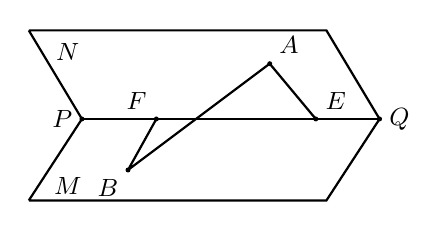
\begin{tikzpicture}[scale=0.9,>=stealth,font=\small]
  \coordinate (P) at (0,0);
  \coordinate (Q) at (4.2,0);
  \coordinate (N1) at (-0.75,1.25);
  \coordinate (N2) at (3.45,1.25);
  \coordinate (M1) at (-0.75,-1.15);
  \coordinate (M2) at (3.45,-1.15);
  \coordinate (A) at (2.65,0.78);
  \coordinate (B) at (0.65,-0.72);
  \coordinate (E) at (3.3,0);
  \coordinate (F) at (1.05,0);
  \draw[thick] (N1)--(N2)--(Q) (P)--(N1);
  \draw[thick] (M1)--(M2)--(Q) (P)--(M1);
  \draw[thick] (P)--(Q);
  \draw[thick] (A)--(B) (A)--(E) (B)--(F);
  \fill (P) circle (1pt) node[left] {$P$};
  \fill (Q) circle (1pt) node[right] {$Q$};
  \fill (A) circle (1pt) node[above right] {$A$};
  \fill (B) circle (1pt) node[below left] {$B$};
  \fill (E) circle (1pt) node[above right] {$E$};
  \fill (F) circle (1pt) node[above left] {$F$};
  \node at (-0.2,0.95) {$N$};
  \node at (-0.2,-0.95) {$M$};
\end{tikzpicture}
